\subsection{Exploring Antenna Modeling: What's Your Analysis Style?}

\begin{tcolorbox}[colback=gray!10, colframe=black, title=E9B09] What type of analysis is commonly used for modeling antennas?
\begin{enumerate}[label=\Alph*)]
    \item A. Graphical analysis
    \item \textbf{B. Method of Moments}
    \item C. Mutual impedance analysis
    \item D. Calculus differentiation with respect to physical properties
\end{enumerate} \end{tcolorbox}

\subsubsection{Concepts Related to Antenna Modeling}

Antenna modeling is a critical aspect of radio communication and electronics that helps designers predict the performance of antennas in various scenarios. The methods used in antenna analysis can greatly affect the design and functionality of an antenna. 

Among the multiple choices given, the \textbf{Method of Moments:} is a well-established technique for solving integral equations that describe the electromagnetic fields around antennas. This method converts the continuous problem of antenna radiation into a discrete system of equations which can be easily solved numerically. 

\subsubsection{Additional Analysis Techniques}

1. \textbf{Graphical Analysis:}: This is more of a visual approach used primarily for illustrative purposes rather than rigorous analysis of antennas. It does not yield precise models or predictions.

2. \textbf{Mutual Impedance Analysis:}: This technique is commonly used in analyzing the interaction between different antennas, but it is not primarily a standalone method of modeling.

3. \textbf{Calculus Differentiation with Respect to Physical Properties:}: While calculus is indeed fundamental to understanding changes in a system, the specific application of differentiation to model antennas is very limited.

\subsubsection{Mathematical Derivation}

To illustrate how the Method of Moments works, let us consider a simple case where we want to analyze a linear dipole antenna. The current distribution can be expressed as \(I(x)\), where \(x\) is the position along the length of the dipole. The electromagnetic fields around the antenna can be determined using:

\[
\mathbf{E}(r, \theta) = \frac{1}{4\pi\epsilon_0} \int_{-L/2}^{L/2} I(x) \cdot G(r, \theta, x) \, dx
\]

where \(G(r, \theta, x)\) is the Green's function representing the influence of an element \( dx \) on the field at point \( (r, \theta) \), and \(\epsilon_0\) is the permittivity of free space.

The correct interpretation and application of the Method of Moments allow engineers to accurately predict radiation patterns and impedance characteristics of various antenna designs.

\subsubsection{Visualization Using TikZ}

To visualize the concept of an antenna and its radiation pattern, we can draw a simple diagram using TikZ as follows:

\begin{center}
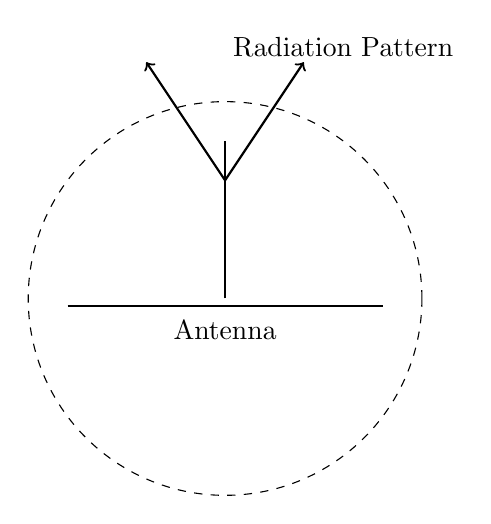
\begin{tikzpicture}
    % Draw the antenna
    \draw[thick] (0,0) -- (0,2);
    
    % Draw ground
    \draw[thick] (-2,-0.1) -- (2,-0.1);
    
    % Draw radiation pattern
    \draw[->, thick] (0,1.5) -- (1,3);
    \draw[->, thick] (0,1.5) -- (-1,3);
    \draw[dashed] (0,0) circle (2.5);
    \node at (0,-0.4) {Antenna};
    \node at (1.5,3.2) {Radiation Pattern};
\end{tikzpicture}
\end{center}
